\section{Pipeline CI/CD}
\label{sec:Pipeline_CICD}

Rozdział opisuje implementację zautomatyzowanego pipeline CI/CD dla modeli uczenia maszynowego. Prezentowane rozwiązanie realizuje przepływ: dodanie danych treningowych przez użytkownika wyzwala sekwencję kroków --- walidację, trening, ocenę jakości i wdrożenie --- bez konieczności ręcznej interwencji.

\subsection{Hook pre-push}

Pierwszym elementem pipeline jest hook Git \texttt{pre-push} \cite{chacon2014pro_git}, instalowany lokalnie na maszynie użytkownika przez skrypt \texttt{devops/scripts/install-git-hooks.sh}. Hook uruchamia się automatycznie przed każdym \texttt{git push} i sprawdza, czy w zestawie zmian znajdują się pliki w katalogach \texttt{WMS/data/training/images/} lub \texttt{WMS/data/training/masks/}.

Jeśli zmiany dotyczą danych treningowych, hook:
\begin{enumerate}
  \item tworzy nową gałąź o nazwie \texttt{data/TIMESTAMP} (np. \texttt{data/20260215-143022}),
  \item commituje do niej wyłącznie nowe pliki z katalogów danych,
  \item przekierowuje push na tę gałąź zamiast na \texttt{main}.
\end{enumerate}

Całość wykonuje się w mniej niż 10 sekund, ponieważ hook nie wymaga połączenia z AWS ani lokalnych poświadczeń chmurowych. Merge danych z historycznym zbiorem w S3 odbywa się po stronie GitHub Actions.

\begin{figure}[H]
  \centering
  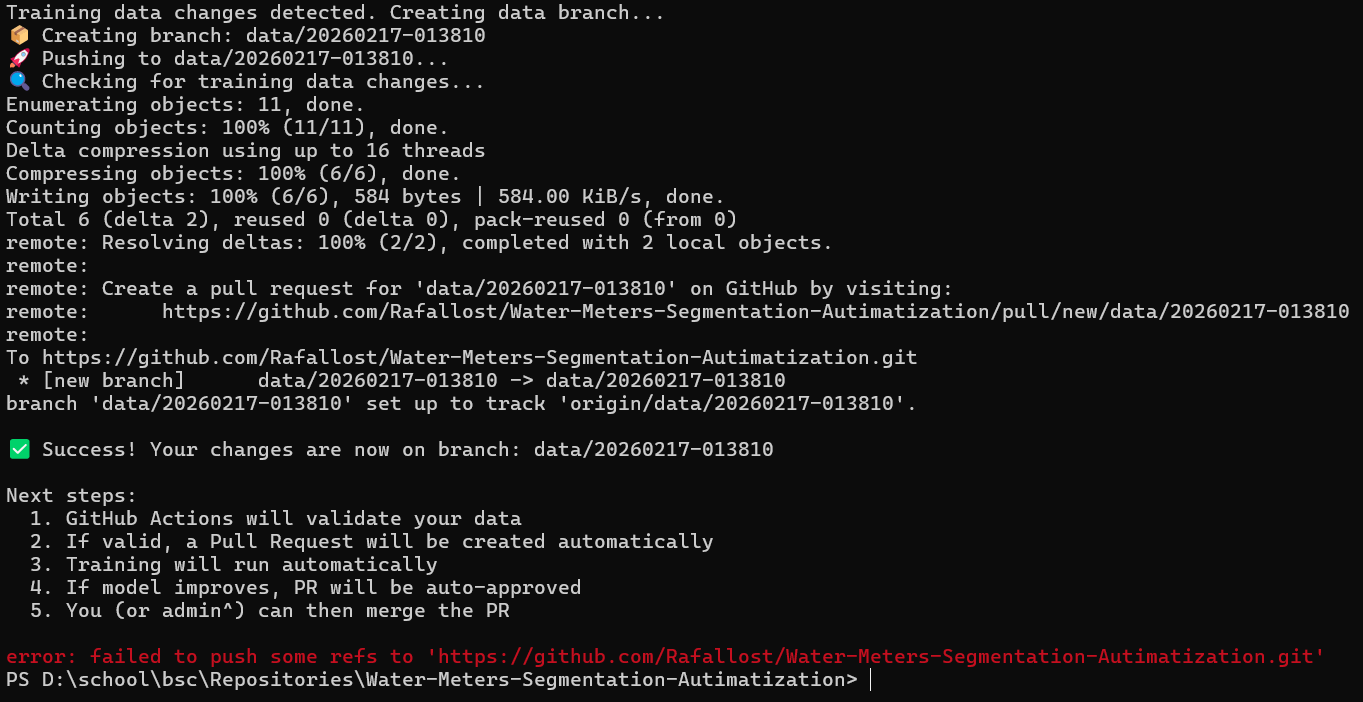
\includegraphics[width=\linewidth]{img/05_pipline_ci_cd/hook.png}
  \caption{Wynik wypchania nowych danych na gałąź \texttt{data/TIMESTAMP}.}
\end{figure}

\subsection{Walidacja danych}

\begin{sloppypar}
Po wypchnięciu gałęzi danych uruchamia się pierwszy job workflow \texttt{training-data-pipeline.yaml} \cite{github_actions_docs}: \texttt{merge-and-validate}. Składa się on z dwóch faz.
\end{sloppypar}

\paragraph{Faza scalania}\mbox{}\\
Job pobiera istniejące dane z Amazon S3 (za pomocą poświadczeń przechowywanych w sekretach GitHub), scala je z nowo dostarczonymi plikami i aktualizuje manifesty DVC. Scalanie jest idempotentne --- pliki o identycznej nazwie i sumie kontrolnej nie są duplikowane.

\paragraph{Faza walidacji}\mbox{}\\
Skrypt \texttt{validate\_data.py} weryfikuje scalony zbiór danych pod kątem czterech kryteriów:
\begin{itemize}
  \item \textbf{kompletność par} --- dla każdego obrazu w katalogu \texttt{images/} musi istnieć maska o tej samej nazwie w \texttt{masks/} (porównanie po \textit{stem} nazwy pliku),
  \item \textbf{rozdzielczość} --- każdy plik obrazu i maski musi mieć rozdzielczość dokładnie $512 \times 512$ px,
  \item \textbf{binarność masek} --- maski mogą zawierać wyłącznie wartości $0$ i $255$ (brak półprzezroczystości),
  \item \textbf{format pliku} --- akceptowane są formaty \texttt{.jpg} oraz \texttt{.png}.
\end{itemize}

Wynik walidacji jest publikowany jako komentarz w pull requeście. W przypadku błędów komentarz zawiera listę plików niezgodnych z wymaganiami, a dalsze jobe są pomijane (warunkowanie przez \texttt{needs} i \texttt{if: needs.merge-and-validate.outputs.valid == 'true'}).

\begin{verbatim}
# Fragment skryptu walidacji
for img_stem in image_stems:
    if img_stem not in mask_stems:
        errors.append(f"Brak maski dla: {img_stem}")
\end{verbatim}

\begin{figure}[H]
    \centering
    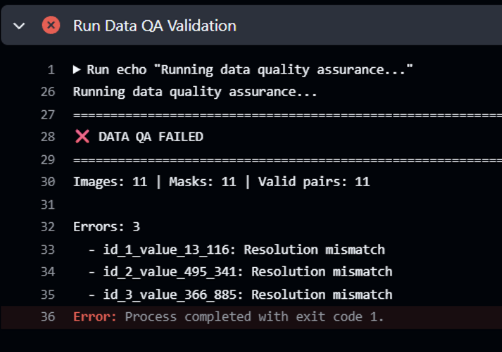
\includegraphics[width=0.7\linewidth]{img/05_pipline_ci_cd/example_qa_stop.png}
    \caption{Przykład komentarza z wynikiem walidacji danych. W tym przypadku wykryto złą rozdzielczość, co skutkuje zatrzymaniem dalszych kroków pipeline.}
    \label{fig:workflow-concurrency}
\end{figure}

\subsection{Pipeline treningowy}

Główny workflow \texttt{training-data-pipeline.yaml} składa się z ośmiu jobów. Joby 1--3 wykonywane są sekwencyjnie. Po zakończeniu treningu workflow rozgałęzia się: gdy model się nie poprawił, uruchamia się \texttt{stop-infra} (job 4); gdy model się poprawił --- równolegle uruchamiają się \texttt{deploy} (job 5) i \texttt{create-pr} (job 7). Job 6 zatrzymuje EC2 po wdrożeniu, a job 8 finalizuje scalenie.

\begin{figure}[H]
    \centering
    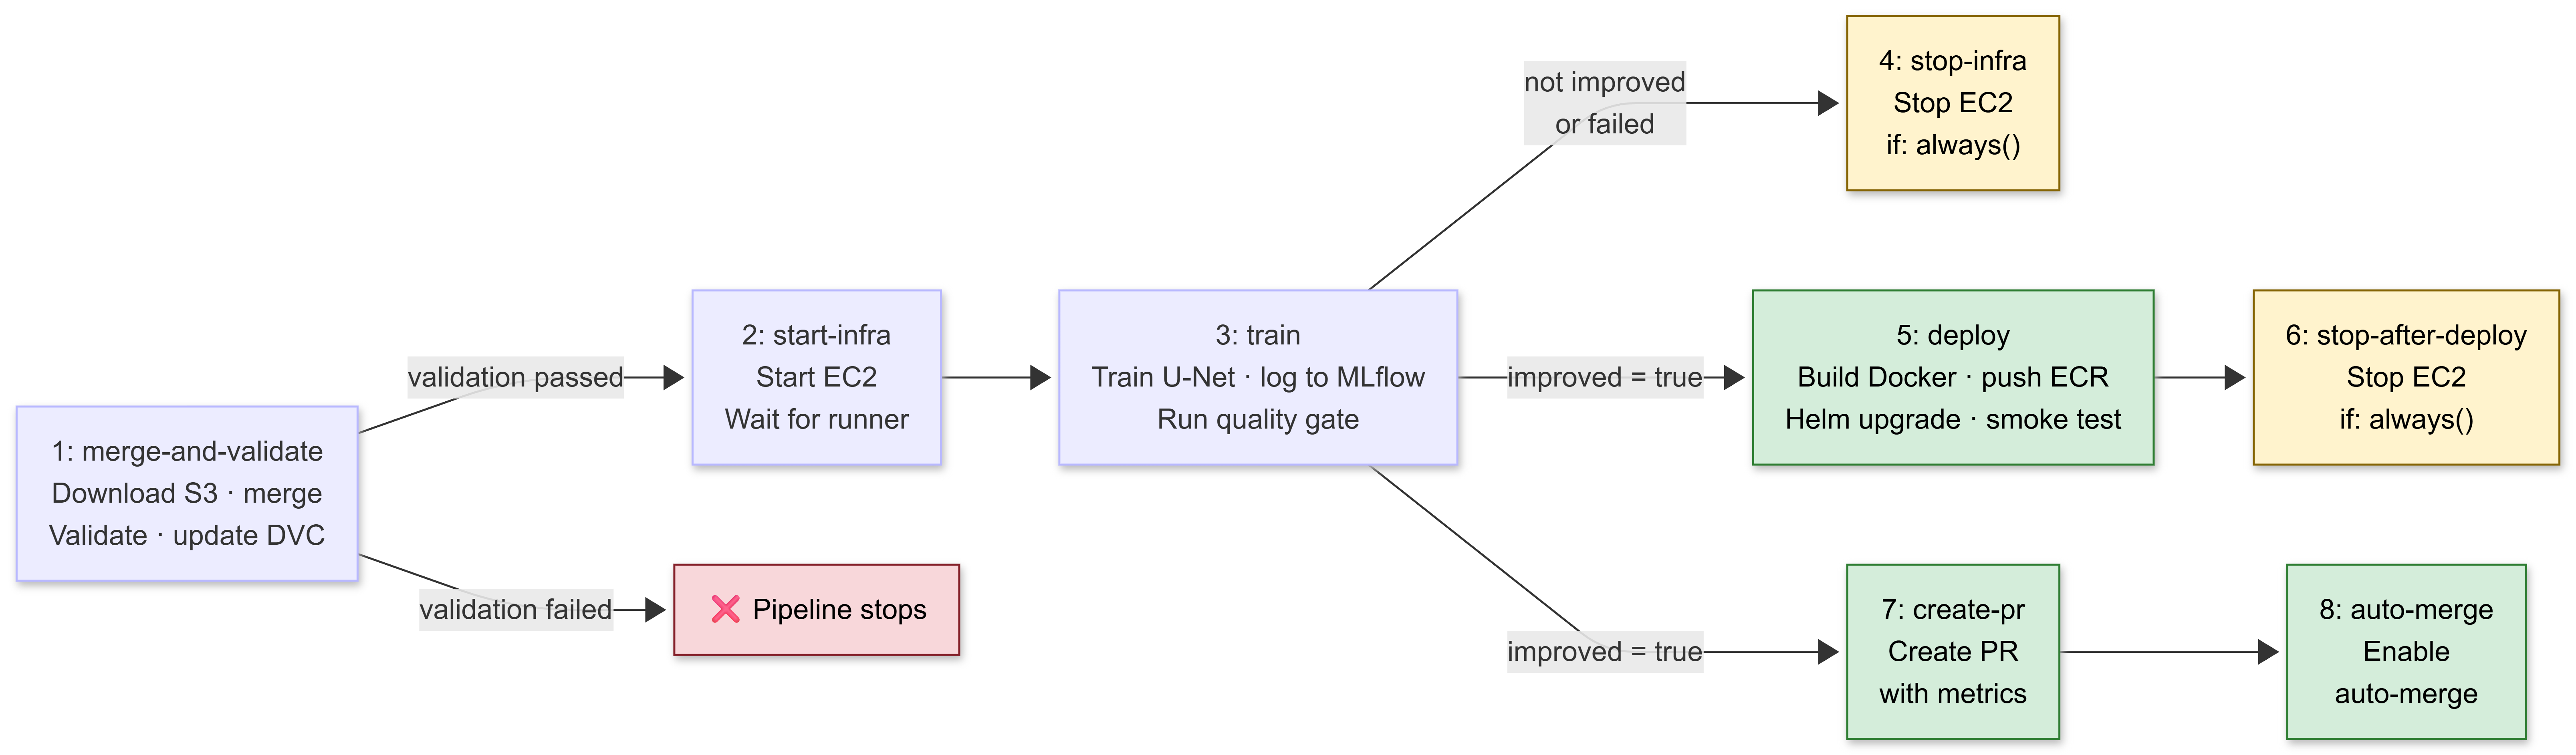
\includegraphics[width=\linewidth]{img/05_pipline_ci_cd/Training_pipline.png}
    \caption{Sekwencja jobów w workflow \texttt{training-data-pipeline.yaml}}
    \label{fig:workflow-jobs}
\end{figure}

\paragraph{Job 1: merge-and-validate}\mbox{}\\
Opracowane we wcześniejszym fragmencie. Pobiera istniejące dane z S3, scala je z nowo dostarczonymi plikami, uruchamia walidację, aktualizuje manifesty DVC i przesyła scalony zbiór jako artefakt GitHub Actions..

\paragraph{Job 2: start-infra}\mbox{}\\
Wykonuje się na hoście GitHub (nie na EC2) i jest odpowiedzialny wyłącznie za uruchomienie infrastruktury. Wywołuje AWS CLI (\texttt{aws ec2 start-instances}) z identyfikatorem instancji zapisanym w sekretach repozytorium. Po wysłaniu polecenia co 30 sekund sprawdza API GitHub, czy self-hosted runner przypisany do tej instancji pojawił się w stanie \textit{online} --- czeka maksymalnie 10 minut. Dzięki temu każdy kolejny job pewnie trafi na już działającą instancję.

\paragraph{Job 3: train}\mbox{}\\
Jedyny job wykonywany na self-hosted runnerze, czyli bezpośrednio na instancji EC2. Pobiera scalony zbiór danych z artefaktu GitHub Actions, uruchamia skrypt \texttt{train.py}, który inicjalizuje model U-Net z seedem równym numerowi uruchomienia (\texttt{run\_number}), trenuje przez zdefiniowaną liczbę epok i loguje metryki \texttt{val\_dice} oraz \texttt{val\_iou} do MLflow. Po zakończeniu treningu skrypt \texttt{quality\_gate.py} pobiera metryki aktualnego modelu Production z rejestru MLflow, porównuje je z wynikami nowego treningu i ustawia output \texttt{improved=true} lub \texttt{improved=false}, sterując dalszym przebiegiem workflow.

\paragraph{Job 4: stop-infra}\mbox{}\\
Zatrzymuje instancję EC2 gdy trening zakończył się błędem lub model nie poprawił wyników (\texttt{if: always() \&\& (train.result != 'success' || improved != 'true')}). Jest to reużywalny workflow wywołujący \texttt{aws ec2 stop-instances}. Dzięki warunkowi \texttt{always()} job uruchamia się nawet gdy poprzednie jobe zakończyły się wyjątkiem, eliminując ryzyko pozostawienia uruchomionej instancji i nieoczekiwanych kosztów.

\paragraph{Job 5: deploy}\mbox{}\\
Uruchamia się wyłącznie jeśli model spełnił kryteria bramki jakości (\texttt{if: improved == 'true'}). Wykonuje się na self-hosted runnerze na EC2. Buduje obraz Docker na podstawie \texttt{docker/Dockerfile.serve}, taguje go numerem wersji i hashiem commita, uwierzytelnia się w Amazon ECR i wgrywa obraz. Następnie wywołuje \texttt{helm upgrade}, który zaktualizuje deployment na klastrze k3s do nowej wersji obrazu --- kontener przy starcie pobiera model ze stadium Production z rejestru MLflow, co oddziela wersję obrazu od wersji modelu. Po wdrożeniu wykonywany jest smoke test sprawdzający dostępność endpointów \texttt{/health}, \texttt{/predict} i \texttt{/metrics}.

\paragraph{Job 6: stop-after-deploy}\mbox{}\\
Zatrzymuje instancję EC2 po zakończeniu joba \texttt{deploy} (\texttt{if: always()}). Stanowi odpowiednik \texttt{stop-infra} dla ścieżki, gdy model się poprawił. Istnieje jako osobny job, ponieważ \texttt{deploy} korzysta z runnera na EC2 --- instancja musi pozostać uruchomiona do końca wdrożenia i może zostać zatrzymana dopiero po jego zakończeniu.

\paragraph{Job 7: create-pr}\mbox{}\\
Uruchamia się równolegle z jobem \texttt{deploy}, jeśli model spełnił kryteria bramki jakości. Tworzy pull request z gałęzi danych do \texttt{main} z automatycznie generowanym opisem zawierającym zestawienie metryk: wartości \texttt{val\_dice} i \texttt{val\_iou} nowego modelu oraz poprzedniego baseline, a także link do uruchomienia MLflow. Pull request scala zaktualizowane manifesty DVC (\texttt{images.dvc}, \texttt{masks.dvc}) z gałęzią główną, trwale łącząc wersję kodu z wersją danych.

\paragraph{Job 8: auto-merge}\mbox{}\\
Włącza automatyczne scalanie pull requesta przez API GitHub (\texttt{gh pr merge --auto}). Scalenie następuje natychmiast po pozytywnym przejściu statusowych sprawdzeń wymaganych przez reguły ochrony gałęzi. W efekcie, jeśli model się poprawił, cały cykl --- od wypchnięcia danych do scalenia z \texttt{main} --- odbywa się bez żadnej ręcznej interwencji.

\begin{figure}[H]
    \centering
    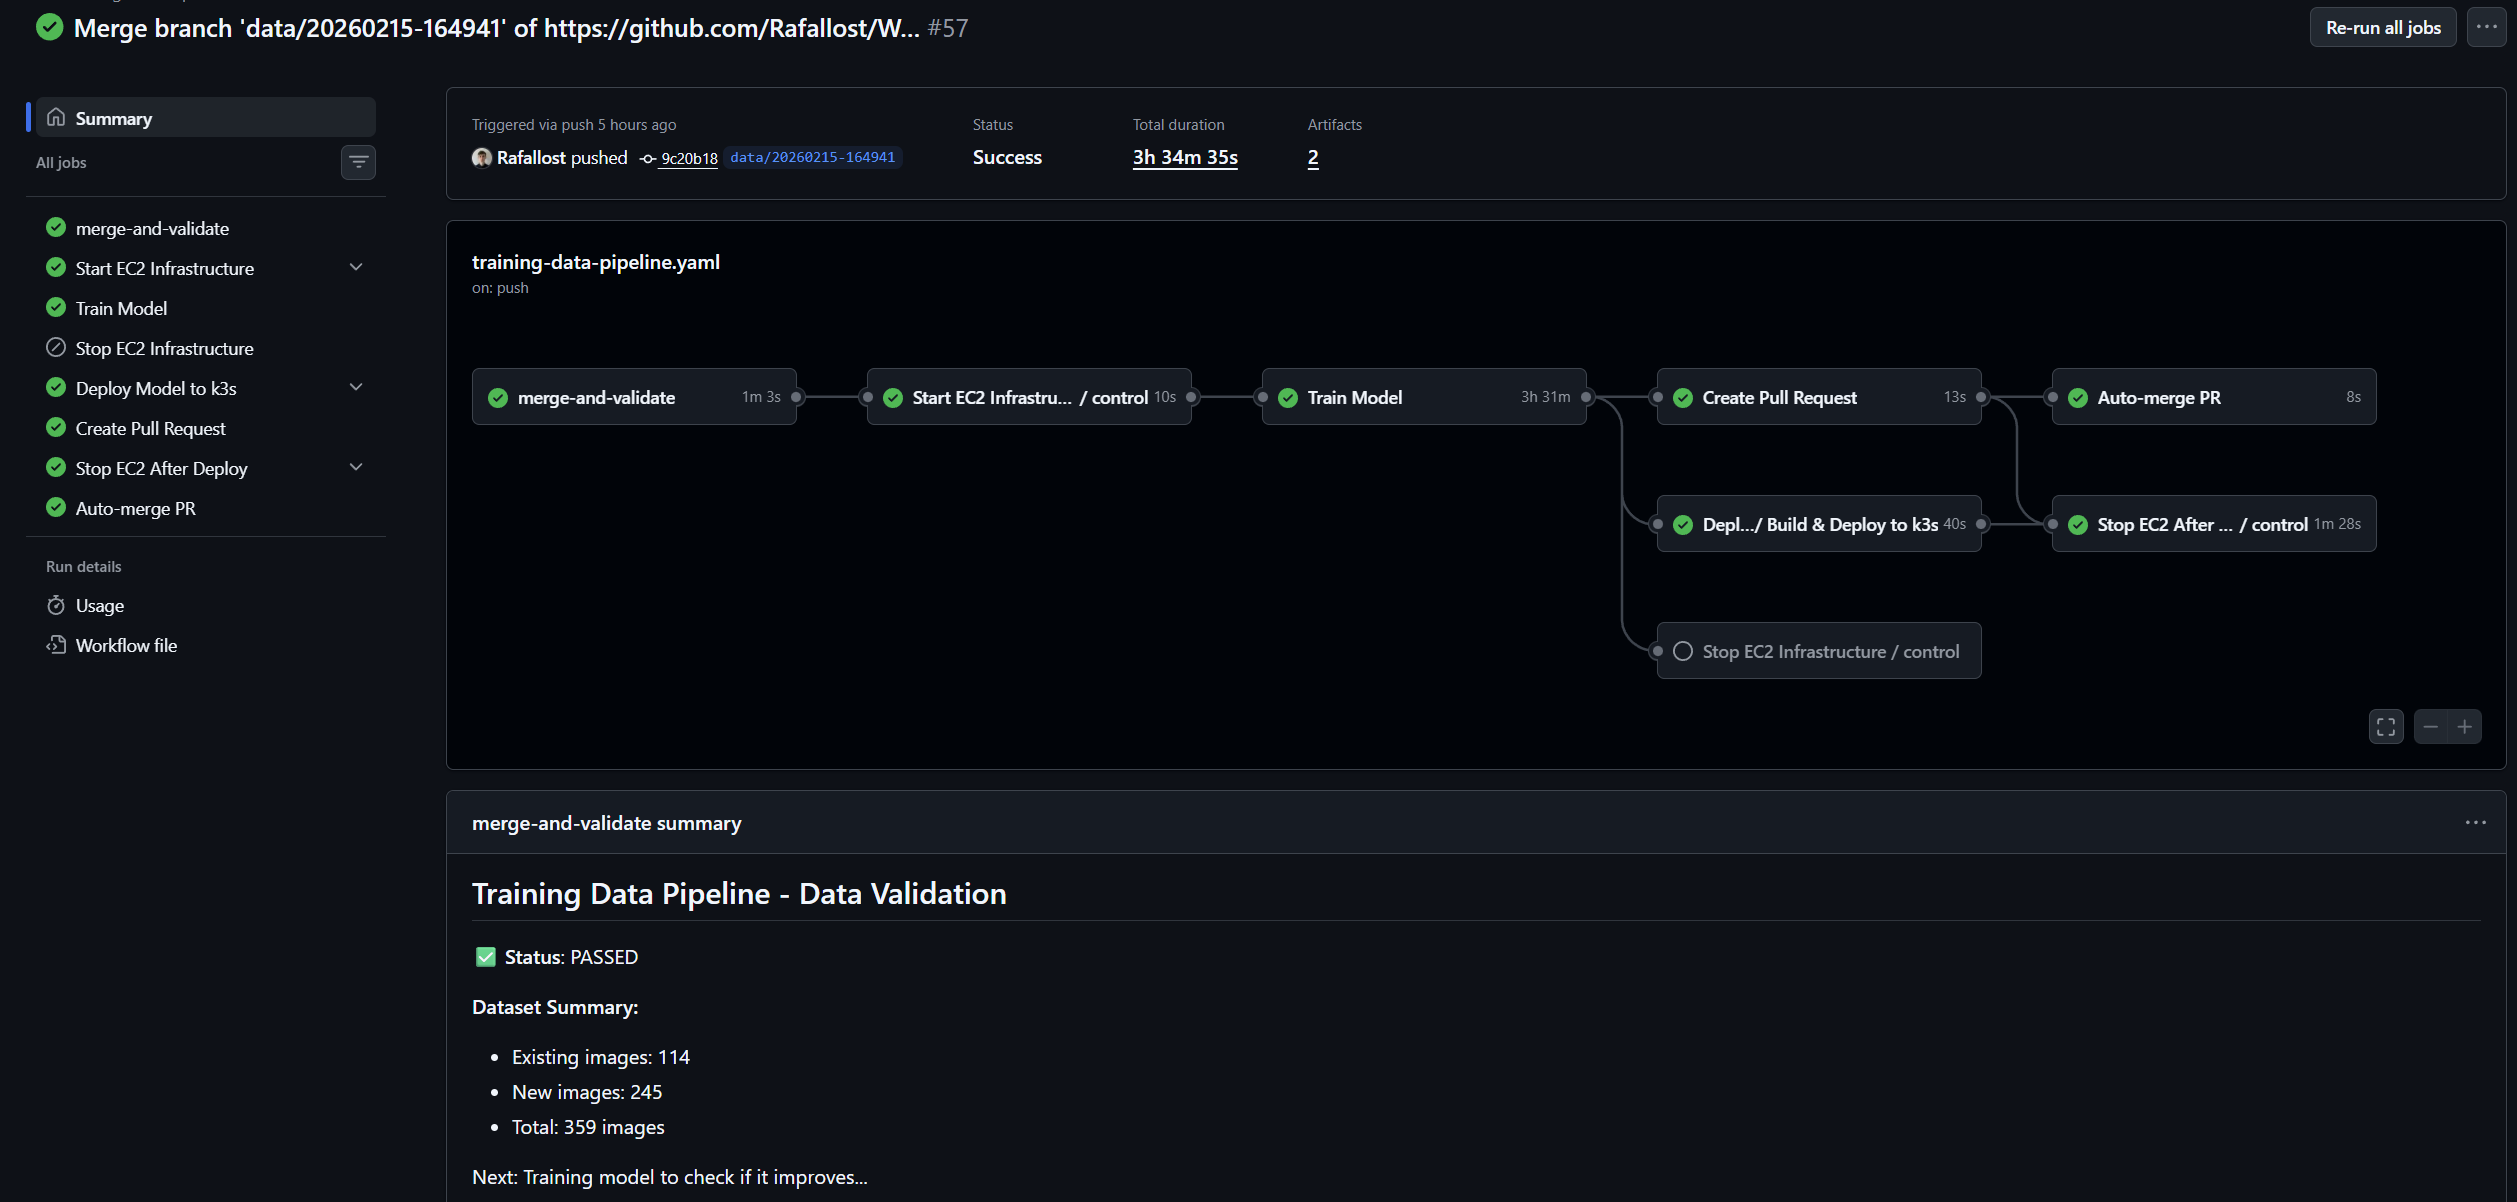
\includegraphics[width=1.0\linewidth]{img/05_pipline_ci_cd/successfull_training.png}
    \caption{Udany przebieg pipeline CI/CD z automatycznym wdrożeniem nowej wersji modelu.}
    \label{fig:workflow-success}
\end{figure}

\subsection{Współbieżność i kolejkowanie}

Workflow skonfigurowany jest z kluczem \texttt{concurrency.cancel-in-progress: false}. Oznacza to, że jeśli użytkownik wypchnął dane kilkakrotnie zanim poprzednie uruchomienie zdążyło się zakończyć, kolejne uruchomienia nie są anulowane --- trafiają do kolejki i wykonują się po zakończeniu poprzednich. Podejście to chroni przed sytuacją, w której późniejszy push nadpisze wyniki wcześniejszego treningu, zanim zostanie on oceniony przez bramkę jakości.

\begin{figure}[H]
    \centering
    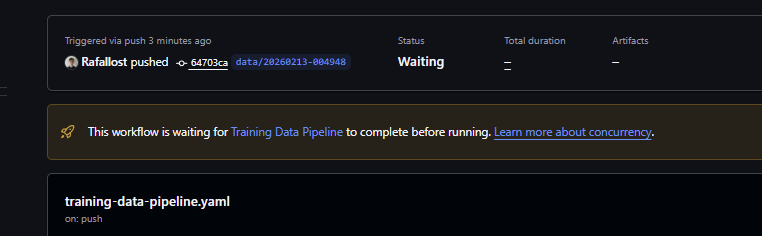
\includegraphics[width=1.0\linewidth]{img/05_pipline_ci_cd/concurrency.png}
    \caption{Kolejkowanie uruchomień workflow w GitHub Actions --- nowe uruchomienie czeka na zakończenie poprzedniego.}
    \label{fig:workflow-concurrency}
\end{figure}

\subsection{Bramka jakości}

Bramka jakości jest mechanizmem decydującym, czy nowy model jest wystarczająco dobry, żeby trafić do produkcji. Implementacja jest w skrypcie \texttt{quality\_gate.py} i korzysta z API MLflow Model Registry \cite{mlflow_model_registry}.

\paragraph{Pobieranie baseline}\mbox{}\\
Skrypt łączy się z MLflow przez \texttt{MlflowClient} i pobiera metryki aktualnego modelu Production:

\begin{verbatim}
client = MlflowClient(tracking_uri=mlflow_uri)
versions = client.get_latest_versions(
    "water-meter-segmentation",
    stages=["Production"]
)
if versions:
    baseline_run = client.get_run(versions[0].run_id)
    baseline_dice = float(
        baseline_run.data.metrics["val_dice"]
    )
else:
    baseline_dice = 0.0  # pierwsze trenowanie
\end{verbatim}

\paragraph{Logika decyzyjna}\mbox{}\\
Model jest uznany za ulepszony, jeśli obie metryki walidacyjne są wyższe od baseline:

\begin{itemize}
  \item \texttt{val\_dice > baseline\_dice}
  \item \texttt{val\_iou > baseline\_iou}
\end{itemize}

Jeśli warunek jest spełniony, skrypt promuje nowy model do etapu Production w MLflow i archiwizuje poprzednią wersję. Wynik jest przekazywany jako output do GitHub Actions (\texttt{echo "improved=true" >> \$GITHUB\_OUTPUT}).

\subsection{Automatyczne wdrożenie}

Gdy bramka jakości potwierdzi poprawę modelu, job \texttt{deploy} w tym samym workflow buduje i wdraża nowy obraz Docker na klastrze k3s --- równolegle z tworzeniem pull requesta (job \texttt{create-pr}).

\paragraph{Budowanie obrazu}\mbox{}\\
Obraz jest budowany na podstawie pliku \texttt{docker/Dockerfile.serve}. Używa warstwy bazowej z PyTorch CPU, kopiuje kod API i instaluje zależności z \texttt{requirements.txt}. Po zbudowaniu obraz jest tagowany numerem wersji i hashiem commita, a następnie wysyłany do Amazon ECR.

\paragraph{Wdrożenie Helm}\mbox{}\\
Helm \cite{helm_docs} aktualizuje deployment na klastrze k3s \cite{k3s_docs} nową wersją obrazu. Konfiguracja wdrożenia zdefiniowana jest w \texttt{infrastructure/helm-values.yaml}. Po wdrożeniu automatycznie wykonywany jest smoke test sprawdzający dostępność endpointów \texttt{/health}, \texttt{/predict} i \texttt{/metrics}.